\documentclass[11pt]{exam}
\usepackage{graphicx}

\usepackage{epsfig}

\usepackage{hyperref}

\usepackage[centertags]{amsmath}
%\usepackage{amsfonts}
\usepackage{amssymb}
\usepackage{amsthm}
\usepackage[all]{xy}
\usepackage{newlfont}
\usepackage{amsmath,amssymb,bm,mathtools}
\usepackage{xcolor} %for color
\usepackage{xmpmulti}
%\usetheme{Air}
%\usefonttheme{professionalfonts}
\usepackage{thumbpdf}
\usepackage{wasysym}
\usepackage{upgreek}
\usepackage{ucs}
%\usepackage[utf8]{inputenc}
\usepackage{pgf,pgfarrows,pgfnodes,pgfautomata,pgfheaps,pgfshade}
\usepackage{verbatim}
\usepackage{empheq}
\newcommand*\widefbox[1]{\fbox{\hspace{2em}#1\hspace{2em}}}

\newcommand{\Integer}{\mathbb{Z}}
\newcommand{\Natural}{\mathbb{Z}_{\geq 0}}
\newcommand{\Naturalstar}{\mathbb{Z}_{> 0}}
\newcommand{\Real}{\mathbb{R}}
\newcommand{\Complex}{\mathbb{C}}
\newcommand{\hilbert}{\mathcal{H}}
\newcommand{\BigHilbert}{\bm{\mathcal{H}}}
\newcommand{\innprod}[2]{\langle{#1},{#2}\rangle}
\newcommand{\ginnprod}[2]{\langle\!\langle{#1},{#2}\rangle\!\rangle}
\newcommand{\norm}[1]{\|{#1}\|}
\newcommand{\mrm}[1]{{\mathrm #1}}
\newcommand{\gnorm}[1]{|\!|\!|{#1}|\!|\!|}
\newcommand{\expect}{\mathbb{E}}

\newcommand{\gr}{\selectlanguage{greek}}

%\newcommand{\red}{\color{myred}}
%\newcommand{\blue}{\color{myblue}}
%\newcommand{\black}{\color{myblack}}


%\definecolor{BrickRed}{cmyk}{0,0.89,0.94,0.28}
%\definecolor{pink}{RGB}{255,192,203}

\begin{document}
\centerline{\Large \sc Homework 5}
\pagestyle{empty}

\hrulefill

\vspace{2cm}


{\Large \sc Name:}



\vspace{2cm}



{\Large \sc Student ID:}

\vspace{6cm}

\begin{itemize}
  \item Reasoning and work must be shown to gain partial/full
  credit
  \item Please include the cover-page on your homework PDF with your name and student ID. Failure of doing so is considered bad citizenship. 

 \end{itemize}

\clearpage
\begin{questions}
\question[1--4]{\bf Lecture 7 Questions}:
Consider the following networks:

\begin{parts}
\part (25\%) Calculate the closeness centrality of each of the nodes in this network:
\begin{center}
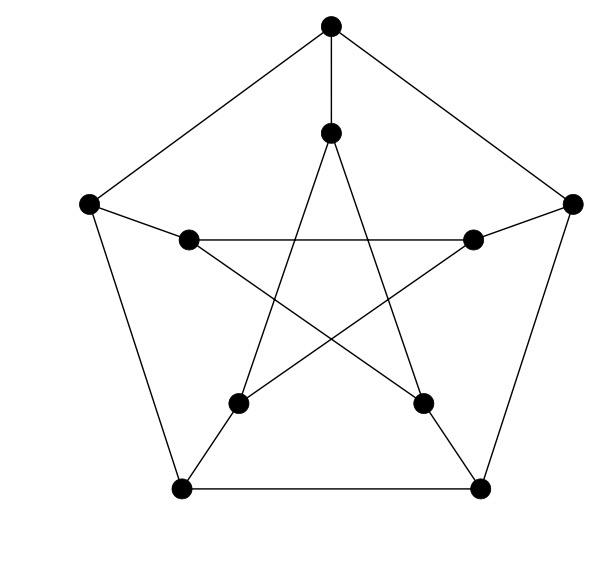
\includegraphics[width=0.4\linewidth]{hw4_1.jpeg}
\end{center}

\part (50\%) Consider these three networks:
\begin{center}
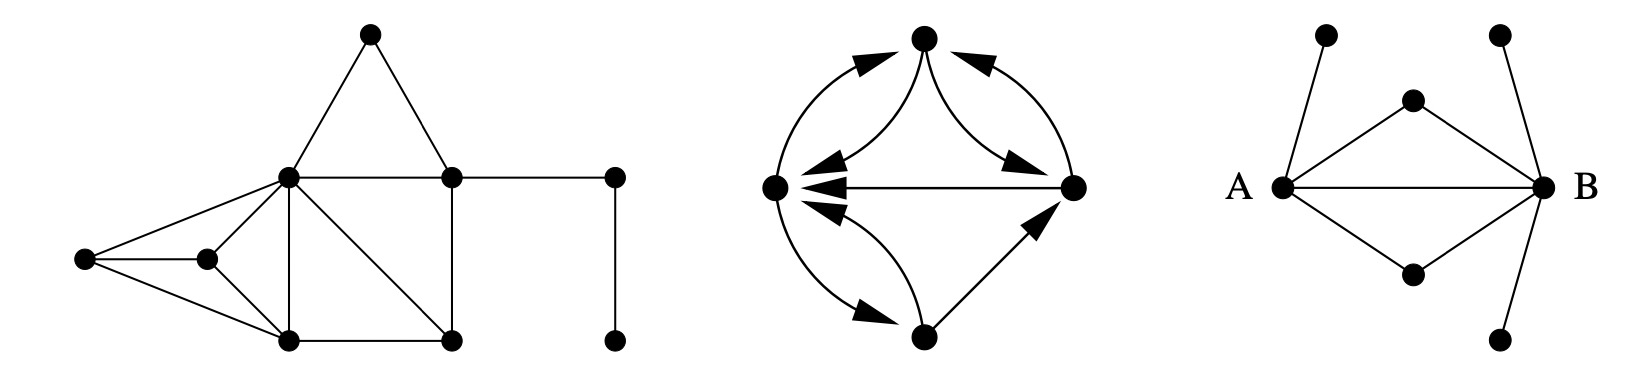
\includegraphics[width=0.9\linewidth]{hw4_2.jpeg}
\end{center}
\begin{enumerate}
\item Find a 3-core in the first network. 
\item What is the reciprocity of the second network? 
\item What is the cosine similarity of nodes A and B in the third network? 
\end{enumerate}


\part (25\%) Calculate the local clustering coefficient of each node in this network:
\begin{center}
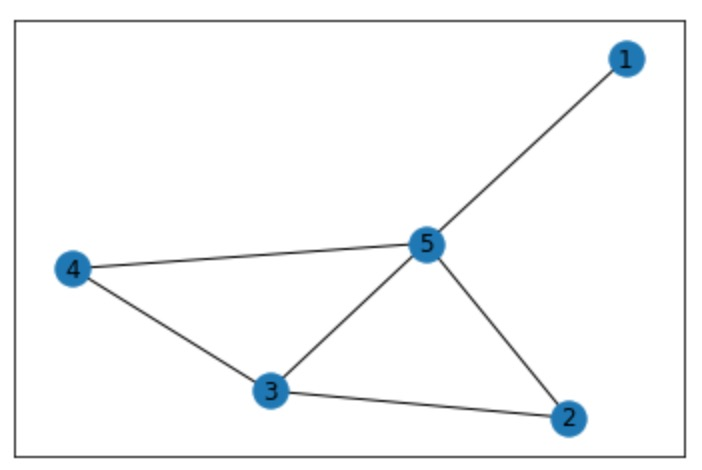
\includegraphics[width=0.75\linewidth]{hw4_3.jpeg}
\end{center}
\end{parts}
\newpage

\question[1--4]{\bf Lecture 8 Questions}:
Consider the random graph $G(n, p)$ with $n$ large.
\begin{parts}
\part (25\%) If the network has a giant component that fills exactly half of the network, what is the average degree of a node?
\part (25\%) For this same random graph what is the probability that a node has degree exactly 5?
\part (25\%) What is the probability that a node belongs to the giant component if it has degree exactly 5? 
\part (25\%) Hence or otherwise, calculate the fraction of nodes in the giant component that have degree exactly 5. 

\end{parts}

\question[1--4]{\bf NetworkX Coding}:
Consider the Erdős-Rényi graph or a binomial graph in NetworkX with the number of nodes $n=20$ and probability for edge creation $p=0.2$ (hint: $G = nx.gnp\_random\_graph(20, 0.2, seed=1096)$).
\begin{parts}
\part Draw this graph and compute transitivity of this graph.
\part Compute  the clustering coefficient for each node and the average clustering coefficient for the graph. 
\part Plot the graph with the colormap of the various metrics of centrality, including  Degree Centrality, Eigenvector Centrality and Closeness Centrality. (See examples of Week4\_tutorials.ipynb in the Canvas.)
\part Compute degree assortativity of graph. 
\part If $p=0.1$, what are the above metrics and what is the minimum $p$ for which you have a giant component?
\end{parts}	



\end{questions}

\end{document}



